%----------------------------------------------------------------------------------------
%
% A LaTeX-template for 1DV510. Modified and translated by Björn Lindenberg at LNU.
% Based on an original master thesis template created by Marcus Wilhelmsson at LNU.
%
%----------------------------------------------------------------------------------------

% Settings and document configuration

\documentclass[a4paper,12pt]{article} 
\usepackage[T1]{fontenc} 
\usepackage{times} 
\usepackage[swedish,english]{babel} 
\usepackage[utf8]{inputenc} 
\usepackage{dtk-logos} 
\usepackage{wallpaper} 
\usepackage[absolute]{textpos} 
\usepackage[top=2cm, bottom=2.5cm, left=3cm, right=3cm]{geometry} 
\usepackage[parfill]{parskip} 
\usepackage{csquotes} 
\usepackage{float} 
\usepackage{lipsum} % Used for dummy text. Can be removed.
\usepackage{listings, color}
\definecolor{mGreen}{rgb}{0,0.6,0}
\definecolor{mGray}{rgb}{0.5,0.5,0.5}
\definecolor{mPurple}{rgb}{0.58,0,0.82}
\definecolor{backgroundColour}{rgb}{0.95,0.95,0.92}

\lstdefinestyle{CStyle}{
    backgroundcolor=\color{backgroundColour},   
    commentstyle=\color{mGreen},
    keywordstyle=\color{magenta},
    numberstyle=\tiny\color{mGray},
    stringstyle=\color{mPurple},
    basicstyle=\footnotesize,
    breakatwhitespace=false,         
    breaklines=true,                 
    captionpos=b,                    
    keepspaces=true,                 
    numbers=left,                    
    numbersep=5pt,                  
    showspaces=false,                
    showstringspaces=false,
    showtabs=false,                  
    tabsize=2,
    language=C
}

% Fontsizes for section headings.
\usepackage{sectsty} 
\sectionfont{\fontsize{14}{15}\selectfont}
\subsectionfont{\fontsize{12}{15}\selectfont}
\subsubsectionfont{\fontsize{12}{15}\selectfont}

%----------------------------------------------------------------------------------------
%	This part is used for the text box on the title page
%----------------------------------------------------------------------------------------
\newsavebox{\mybox}
\newlength{\mydepth}
\newlength{\myheight}

\newenvironment{sidebar}%
{\begin{lrbox}{\mybox}\begin{minipage}{\textwidth}}%
{\end{minipage}\end{lrbox}%
 \settodepth{\mydepth}{\usebox{\mybox}}%
 \settoheight{\myheight}{\usebox{\mybox}}%
 \addtolength{\myheight}{\mydepth}%
 \noindent\makebox[0pt]{\hspace{-20pt}\rule[-\mydepth]{1pt}{\myheight}}%
 \usebox{\mybox}}

%----------------------------------------------------------------------------------------
%	Title
%----------------------------------------------------------------------------------------
\newcommand\BackgroundPic{
    \put(-2,-3){
    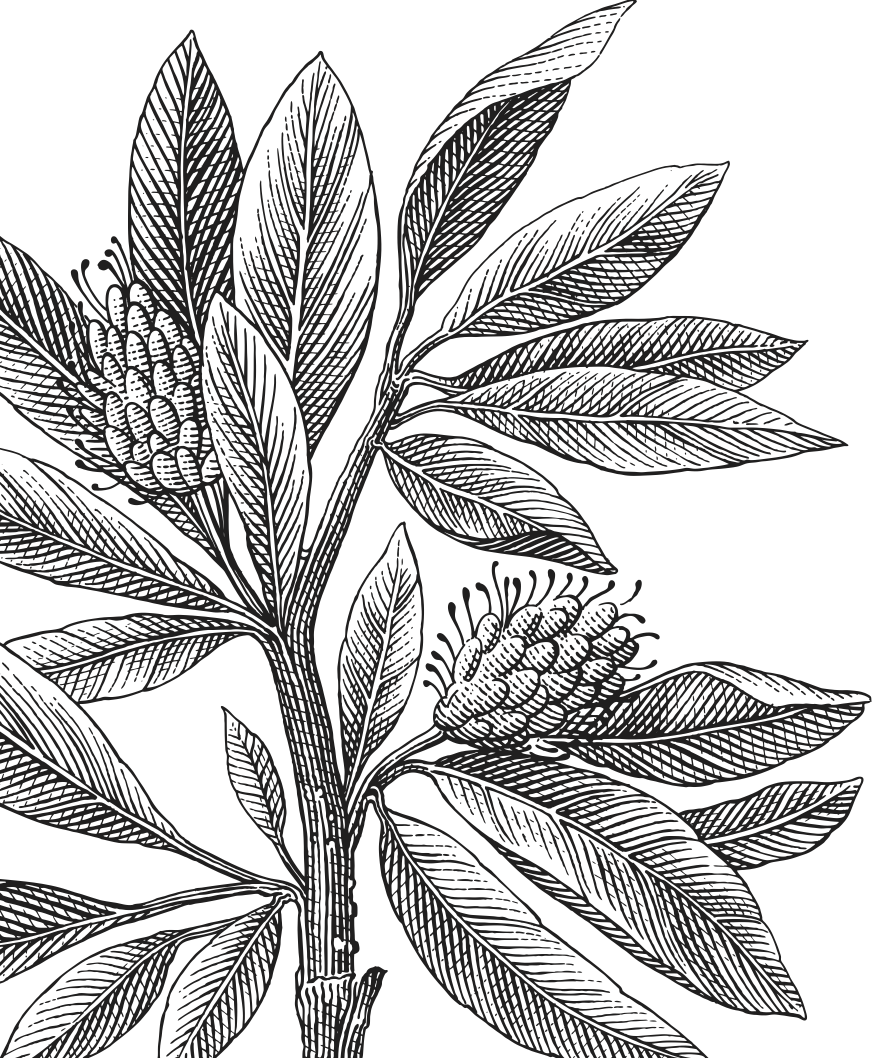
\includegraphics[keepaspectratio,scale=0.3]{img/lnu_etch.png} % Background image
    }
}
\newcommand\BackgroundPicLogo{
    \put(30,740){
    
\includegraphics[keepaspectratio,scale=0.10]{img/logo.png} % LNU logo
    }
}

\title{
\vspace{-8cm}
\begin{sidebar}
    \vspace{10cm}
    \normalfont \normalsize
    \huge Computer Technology I\\ % Main title
    \vspace{-1.3cm}
\end{sidebar}
\vspace{3cm}
\begin{flushleft}
    \huge Lab. 6 : CyberTech Wall Display % Subtitle
     \small \\ \emph{}
\end{flushleft}
\null
\vfill
\begin{textblock}{5}(10,13)
\begin{flushright}
\begin{minipage}{\textwidth}
\begin{flushleft} \large
\emph{Author:}\textsc{Anas Kwefati}\\  % Author
\emph{Supervisor:}  \textsc{Anders Haggren} \\  % Author
\emph{Semester:} Autumn 2019\\ % Semester
\emph{Area:} Computer Science \\ % Area
\emph{Course code:} 1DT301 % Course
\end{flushleft}
\end{minipage}
\end{flushright}
\end{textblock}
}

\date{} % Empty date command. Use \today inside for today's date.
\author{} % Normally one would use this to define authors. However in this case the title command takes care of everything, so we leave the field empty to get rid of warnings. 

\begin{document}

\pagenumbering{gobble} % Turn off page numbering
\newgeometry{left=5cm}
\AddToShipoutPicture*{\BackgroundPic} % Adds the background image to the title page
\AddToShipoutPicture*{\BackgroundPicLogo} % Adds the logo to the title page
\maketitle % Prints the title
\restoregeometry
\clearpage

\pagenumbering{roman} % Roman page numbering for abstract page


\selectlanguage{english}

\newpage

\pagenumbering{gobble} % Turn off page numbering
\tableofcontents 

\newpage
\pagenumbering{arabic} % Turn on page numbering

%TASK1
\section{Task 1}
\lstset{style=CStyle}

\begin{lstlisting}[style=CStyle]
/*>>>>>>>>>>>>>>>>>>>>>>>>>>>>>>>>>>>>>>>>>>>>>>>>>>>>>>>>>>>
; 1DT301, Computer Technology I
; Date: 2016-09-15
; Author:
;    Anas Kwefati
;
; Lab number: 6
; Title: CyberTech Wall Display
;
; Hardware: STK600, CPU ATmega2560
;
; Function: Program that writes a character on the CyberTech Display.
;
; Input ports: none
;
; Output ports: CyberTech Display.
;
; Subroutines:
; Included files: <avr/io.h>
;
;Other information: Display is connected to the serial port (RS232) on the STK600.
; Communication speed is 2400bps.
;Changes in program: (Description and date)
<<<<<<<<<<<<<<<<<<<<<<<<<<<<<<<<<<<<<<<<<<<<<<<<<<<<<<<<<<<*/

#include <avr/io.h>
#include <stdio.h>
#include <string.h>
//#include <util/delay.h>
#define FCPU 1000000// Clock Speed
#define BAUD 2400 //Communication Speed Display rate 2400
#define MYUBBRR (FCPU/16/BAUD-1) //UBBRR = 25 -> osc = 1MHz and UBRR = 47 -> osc = 1,843200MHz

void uart_int(void);
void toPutty(unsigned char data);

int main(void)
{
    uart_int();
    
    char* txt = "\rAO0001Hi How are you ? :)";
    int checksum =0;
    //We make sure that everything is in it
    for(int i =0; i<strlen(txt);i++){
        checksum += txt[i];
    }
    
    checksum\%=256;
    
    char toDisplay [strlen(txt)+3];
    sprintf(toDisplay, "\%s\%02X\n", txt, checksum); //\%02x means print at least 2 digits, prepends it with 0's if there's less.
    //\%02x is used to convert one character to a hexadecimal string
    
    for (int i = 0; i<strlen(txt)+3;i++){
        toPutty(toDisplay[i]);
    }
    
    txt = "\rZD0013C\n";
    for(int i = 0; i<strlen(txt);i++){
        toPutty(txt[i]);
    }
    
    return 0;
}

//INITALIZATION OF THE DISPLAY

void toPutty(unsigned char data){
    //WAIT FOR DATA TO BE RECEIVED
    while(!(UCSR1A & (1<<UDRE1)));
    UDR1 = data;
}

void uart_int(void) {
    UBRR1L = MYUBBRR; //25 because we are setting the board at 1MHz
    /*Enable receiver and transmitter*/
    UCSR1B = (1<<RXEN1|1<<TXEN1); // Receive Enable (RXEN) bit // Transmit Enable (TXEN) bit
}


\end{lstlisting}

\break
\begin{figure}
\begin{center}
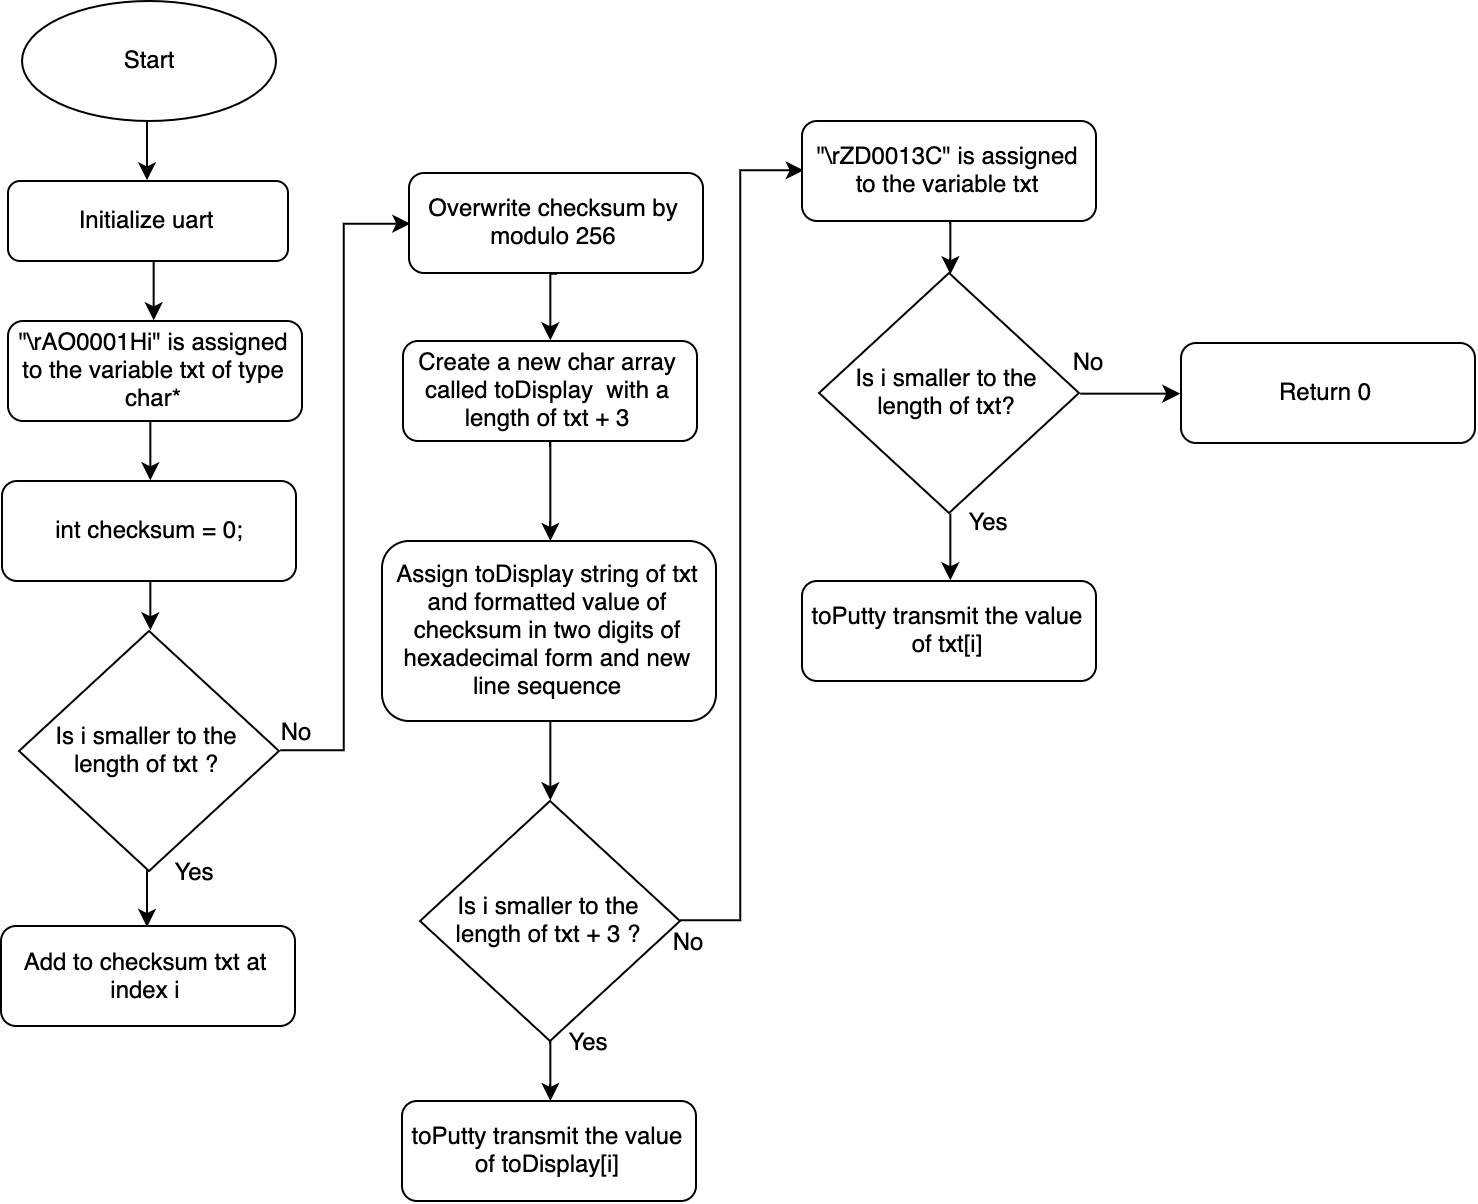
\includegraphics[width=\textwidth/1 ]{flowchart/task1_flowchart.png}
\end{center}
\caption{Task 1 flowchart}
\label{task1}
\end{figure}



%TASK2
\section{Task 2}

\lstset{style=CStyle}

\begin{lstlisting}[style=CStyle]
/*>>>>>>>>>>>>>>>>>>>>>>>>>>>>>>>>>>>>>>>>>>>>>>>>>>>>>>>>>>>
; 1DT301, Computer Technology I
; Date: 2016-09-15
; Author:
;    Anas Kwefati
;
; Lab number: 6
; Title: CyberTech Wall Display
;
; Hardware: STK600, CPU ATmega2560
;
; Function: Program that writes characters on all text lines on the CyberTech Display.
; The program will write to all 3 rows.
;
; Input ports: none
;
; Output ports: CyberTech Display.
;
; Subroutines:
; Included files: <avr/io.h>
;
;Other information: Display is connected to the serial port (RS232) on the STK600.
; Communication speed is 2400bps.
;Changes in program: (Description and date)
<<<<<<<<<<<<<<<<<<<<<<<<<<<<<<<<<<<<<<<<<<<<<<<<<<<<<<<<<<<*/

#include <avr/io.h>
#include <stdio.h>
#include <string.h>
//#include <util/delay.h>
#define FCPU 1000000// Clock Speed
#define BAUD 2400 //Communication Speed Display rate 2400
#define MYUBBRR (FCPU/16/BAUD-1) //UBBRR = 25 -> osc = 1MHz and UBRR = 47 -> osc = 1,843200MHz

void uart_int(void);
void toPutty(unsigned char data);
void toDisplayOnLCD(char* stringChar);

int main(void)
{
	uart_int();
	
	char* txt = "\rAO0001First Line              Second Line";
	
	toDisplayOnLCD(txt);
	

	
	txt = "\rBO0001Third Line";
	toDisplayOnLCD(txt);
	
	txt = "\rZD0013C\n";
	toDisplayOnLCD(txt);
	
	return 0; 
}


//METHOD TO DISPLAY ON THE SCREEN 
void toDisplayOnLCD(char* stringChar){
	
	int checksum = 0; 
	 //We make sure that everything is in it
	 for(int i =0; i<strlen(stringChar);i++){
		 checksum += stringChar[i];
	 }
	 
	 checksum\%=256;
	 
	 char toDisplay [strlen(stringChar)+3];
	 sprintf(toDisplay, "\%s\%02X\n", stringChar, checksum); //\%02x means print at least 2 digits, prepends it with 0's if there's less.
	 //\%02x is used to convert one character to a hexadecimal string
	
	for (int i = 0; i<strlen(stringChar)+3;i++){
		toPutty(toDisplay[i]);
	}
}

//INITIALIZATION OF THE DISPLAY 

void toPutty(unsigned char data){
	//WAIT FOR DATA TO BE RECEIVED
	while(!(UCSR1A & (1<<UDRE1)));
	UDR1 = data;
}

void uart_int(void) { 
	UBRR1L = MYUBBRR; //25 because we are setting the board at 1MHz
	/*Enable receiver and transmitter*/
	UCSR1B = (1<<RXEN1|1<<TXEN1); // Receive Enable (RXEN) bit // Transmit Enable (TXEN) bit
}




\end{lstlisting}
\break
\begin{figure}
\begin{center}
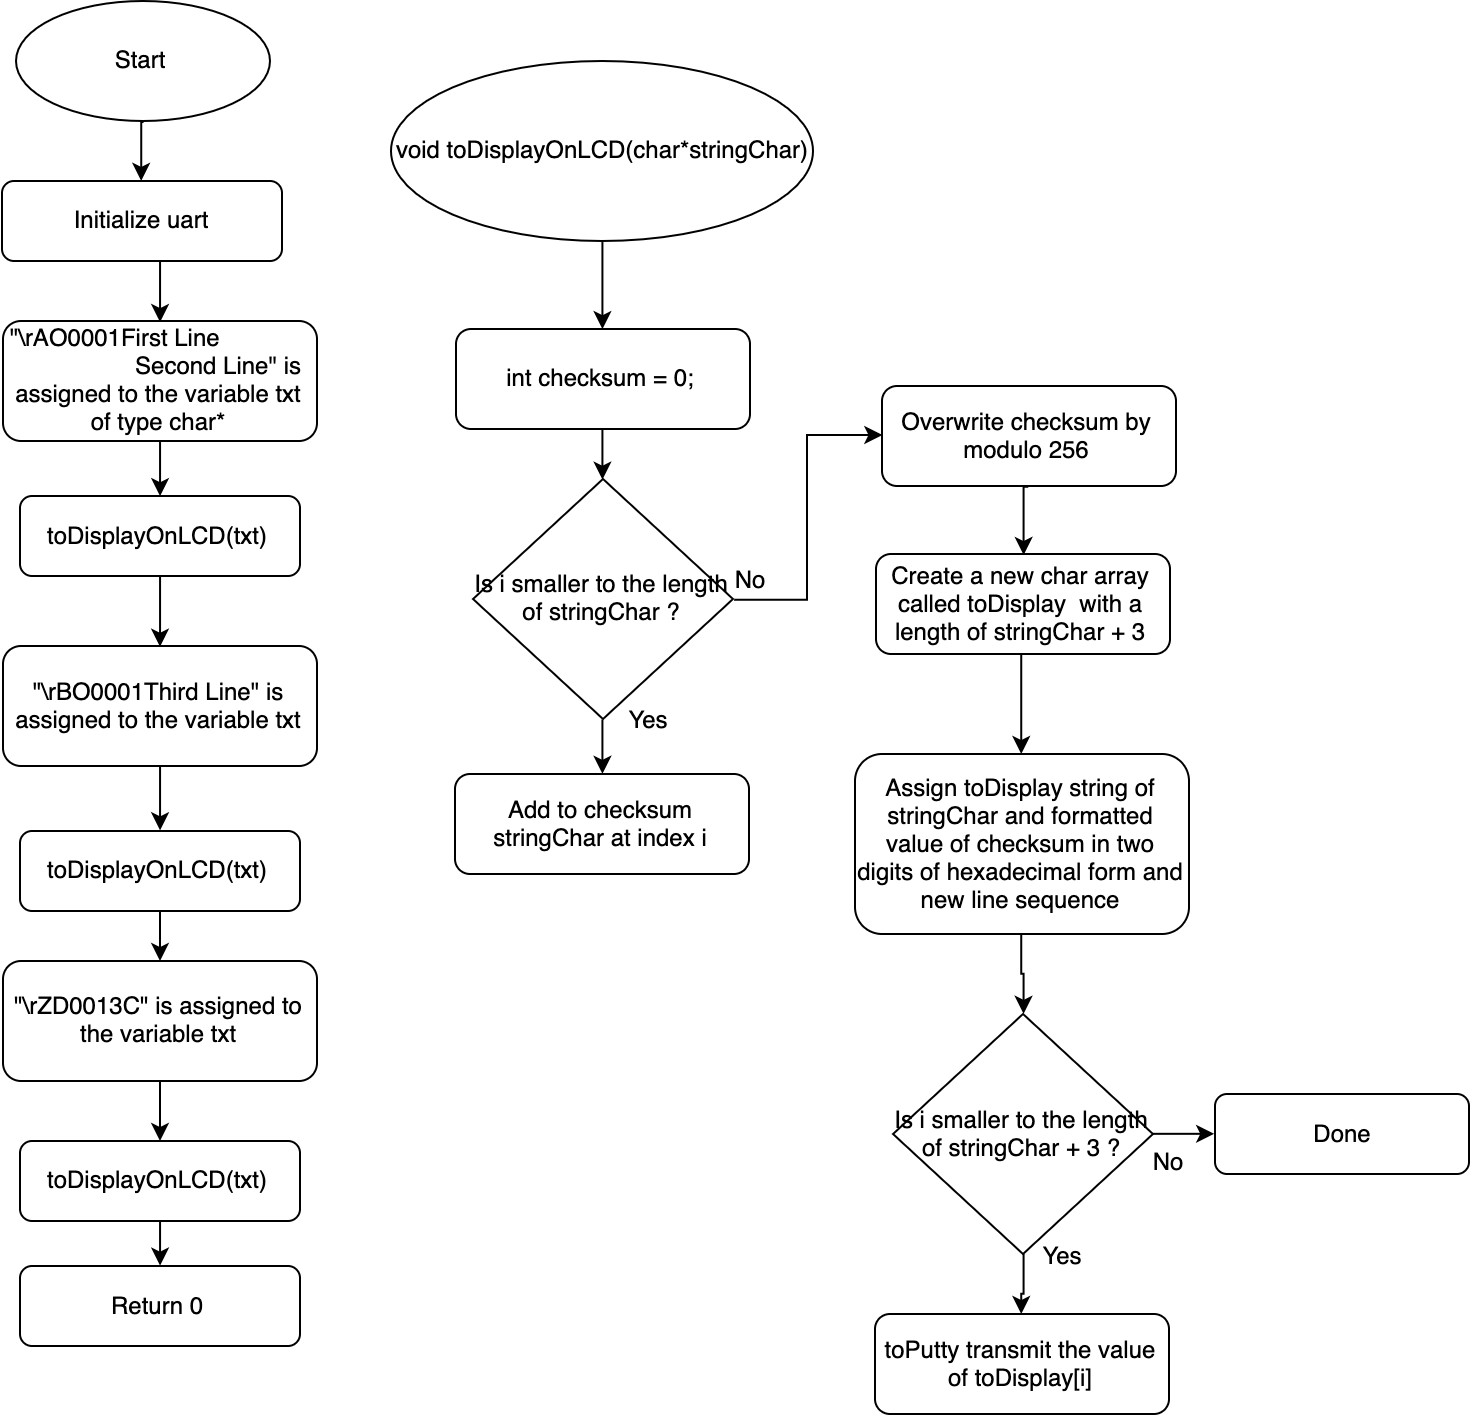
\includegraphics[width=\textwidth/1]{flowchart/task2_flowchart.png}
\end{center}
\caption{Task 2 flowchart}
\label{task2}
\end{figure}

\break

%TASK 3

\section{Task 3}

\lstset{style=CStyle}

\begin{lstlisting}[style=CStyle]
/*>>>>>>>>>>>>>>>>>>>>>>>>>>>>>>>>>>>>>>>>>>>>>>>>>>>>>>>>>>>
; 1DT301, Computer Technology I
; Date: 2016-09-15
; Author:
;    Anas Kwefati
;
; Lab number: 6
; Title: CyberTech Wall Display
;
; Hardware: STK600, CPU ATmega2560
;
; Function: Program that changes text strings on the display.
;
; Input ports: none
;
; Output ports: CyberTech Display.
;
; Subroutines:
; Included files: <avr/io.h> and <util/delay.h>
;
;Other information: Display is connected to the serial port (RS232) on the STK600.
; Communication speed is 2400bps.
;Changes in program: (Description and date)
<<<<<<<<<<<<<<<<<<<<<<<<<<<<<<<<<<<<<<<<<<<<<<<<<<<<<<<<<<<*/
#include <avr/io.h>
#include <stdio.h>
#include <string.h>
#include <stdlib.h>

#define F_CPU 1000000// Clock Speed
#include <util/delay.h>
#define BAUD 2400 //Communication Speed Display rate 2400
#define MYUBBRR (F_CPU/16/BAUD-1) //UBBRR = 25 -> osc = 1MHz and UBRR = 47 -> osc = 1,843200MHz

void uart_int(void);
void toPutty(unsigned char data);
void toDisplayOnLCD(char* stringChar);

int main(void)
{
	uart_int();
	

	char* data = "abc";
	char *txt = "\rAO0001";
	
	for(int i =0;i<strlen(data);i++){
		//The idea is to take char by char and add it one by one to str2
		char c = data[i];
		size_t len = strlen(txt); //take the length of txt
		char *str2 = malloc(len + 1 + 1); //give a length of len and allocate a bit more memory with malloc in case 
		strcpy(str2, txt); // copy txt to str2
		str2[len] = c;  //create an array of str2 with a length of len for the char c
		str2[len + 1] = '\0'; // we add 1 to len and add the end char \0
		toDisplayOnLCD(str2); //call display
		free(str2); //free str2 deallocate the space used by malloc()
		
		str2 = "\rZD0013C";
		toDisplayOnLCD(str2);
		_delay_ms(5000); //wait 5s
	}

		
	return 0; 
}



//METHOD TO DISPLAY ON THE SCREEN 
void toDisplayOnLCD(char* stringChar){
	
	int checksum = 0; 
	 //We make sure that everything is in it
	 for(int i =0; i<strlen(stringChar);i++){
		 checksum += stringChar[i];
	 }
	 
	 checksum\%=256;
	 
	 char toDisplay [strlen(stringChar)+3];
	 sprintf(toDisplay, "\%s\%02X\n", stringChar, checksum); //\%02x means print at least 2 digits, prepends it with 0's if there's less.
	 //\%02x is used to convert one character to a hexadecimal string
	
	for (int i = 0; i<strlen(stringChar)+3;i++){
		toPutty(toDisplay[i]);
	}
}

//INITIALIZATION OF THE DISPLAY 

void toPutty(unsigned char data){
	//WAIT FOR DATA TO BE RECEIVED
	while(!(UCSR1A & (1<<UDRE1)));
	UDR1 = data;
}

void uart_int(void) { 
	UBRR1L = MYUBBRR; //25 because we are setting the board at 1MHz
	/*Enable receiver and transmitter*/
	UCSR1B = (1<<RXEN1|1<<TXEN1); // Receive Enable (RXEN) bit // Transmit Enable (TXEN) bit
}




\end{lstlisting}
\break
\begin{figure}
\begin{center}
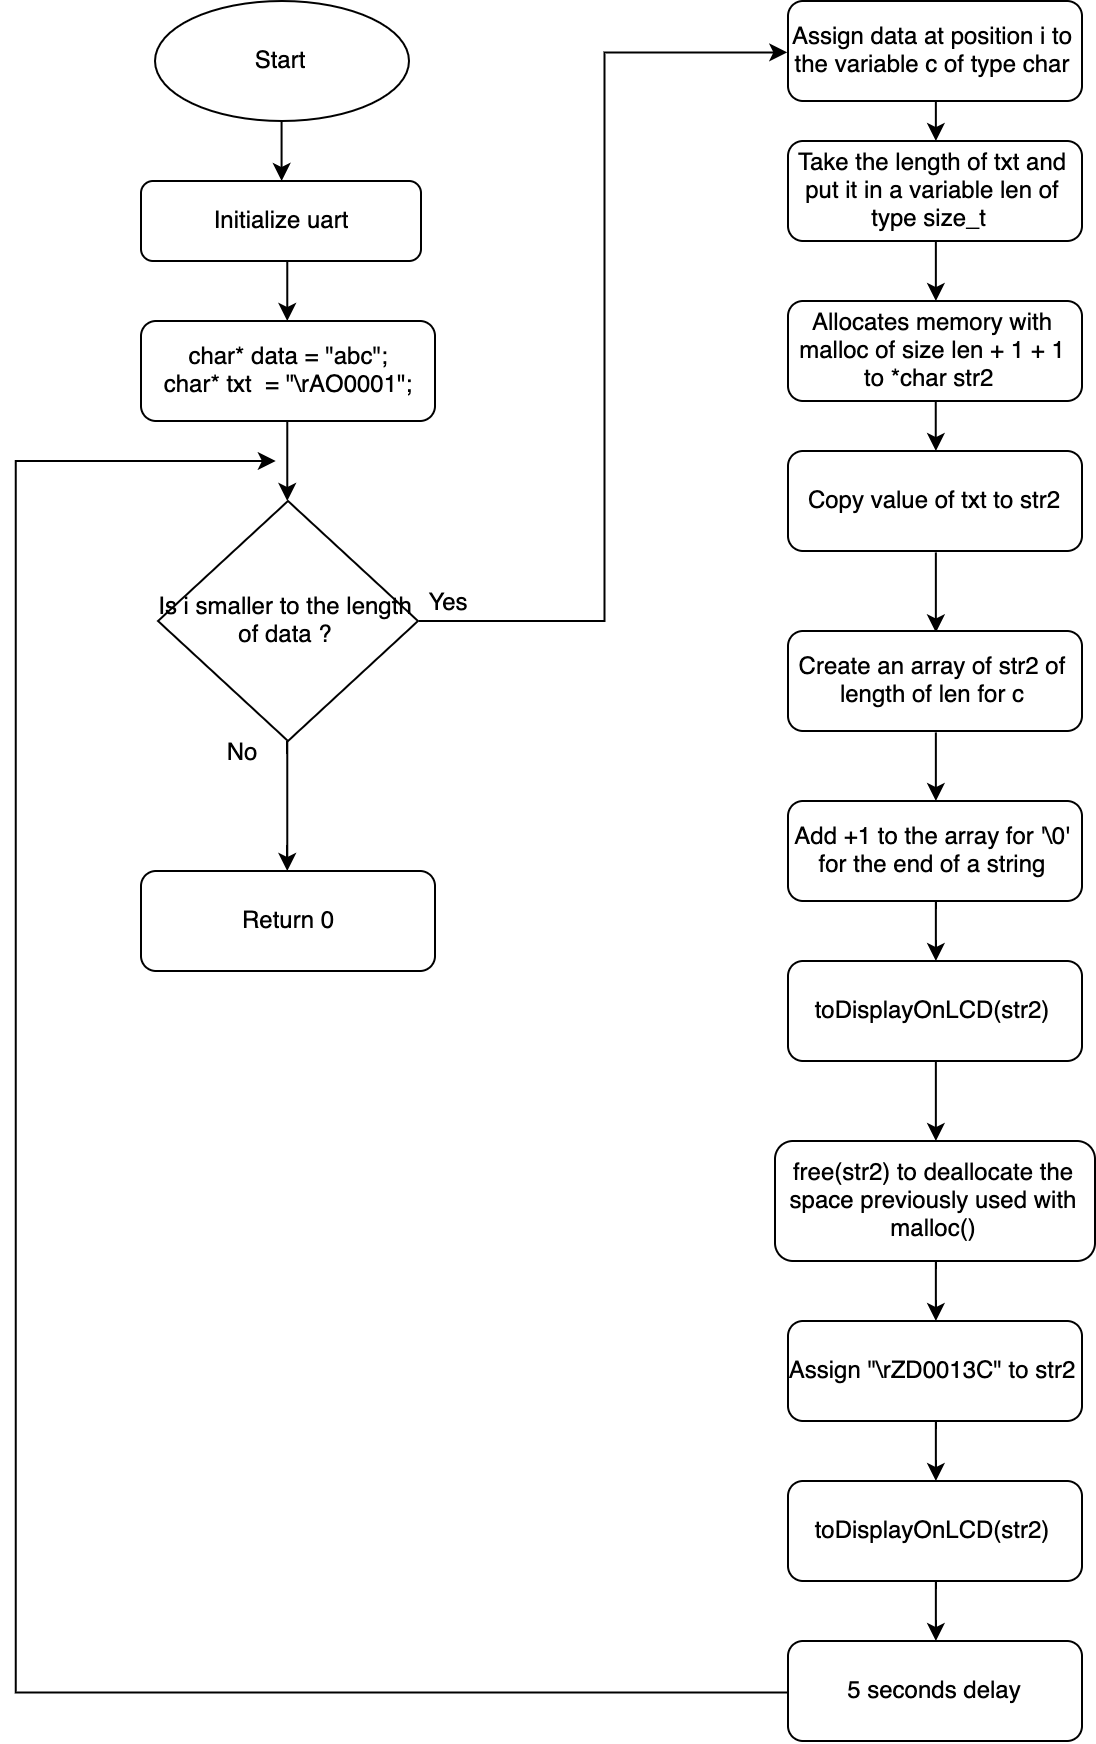
\includegraphics[width=\textwidth/2]{flowchart/task3_flowchart.png}
\end{center}
\caption{Task 3 flowchart}
\label{task3}
\end{figure}

\break

%TASK4
\section{Task 4}

\lstset{style=CStyle}

\begin{lstlisting}[style=CStyle]


\end{lstlisting}

\break
\begin{figure}
\begin{center}
%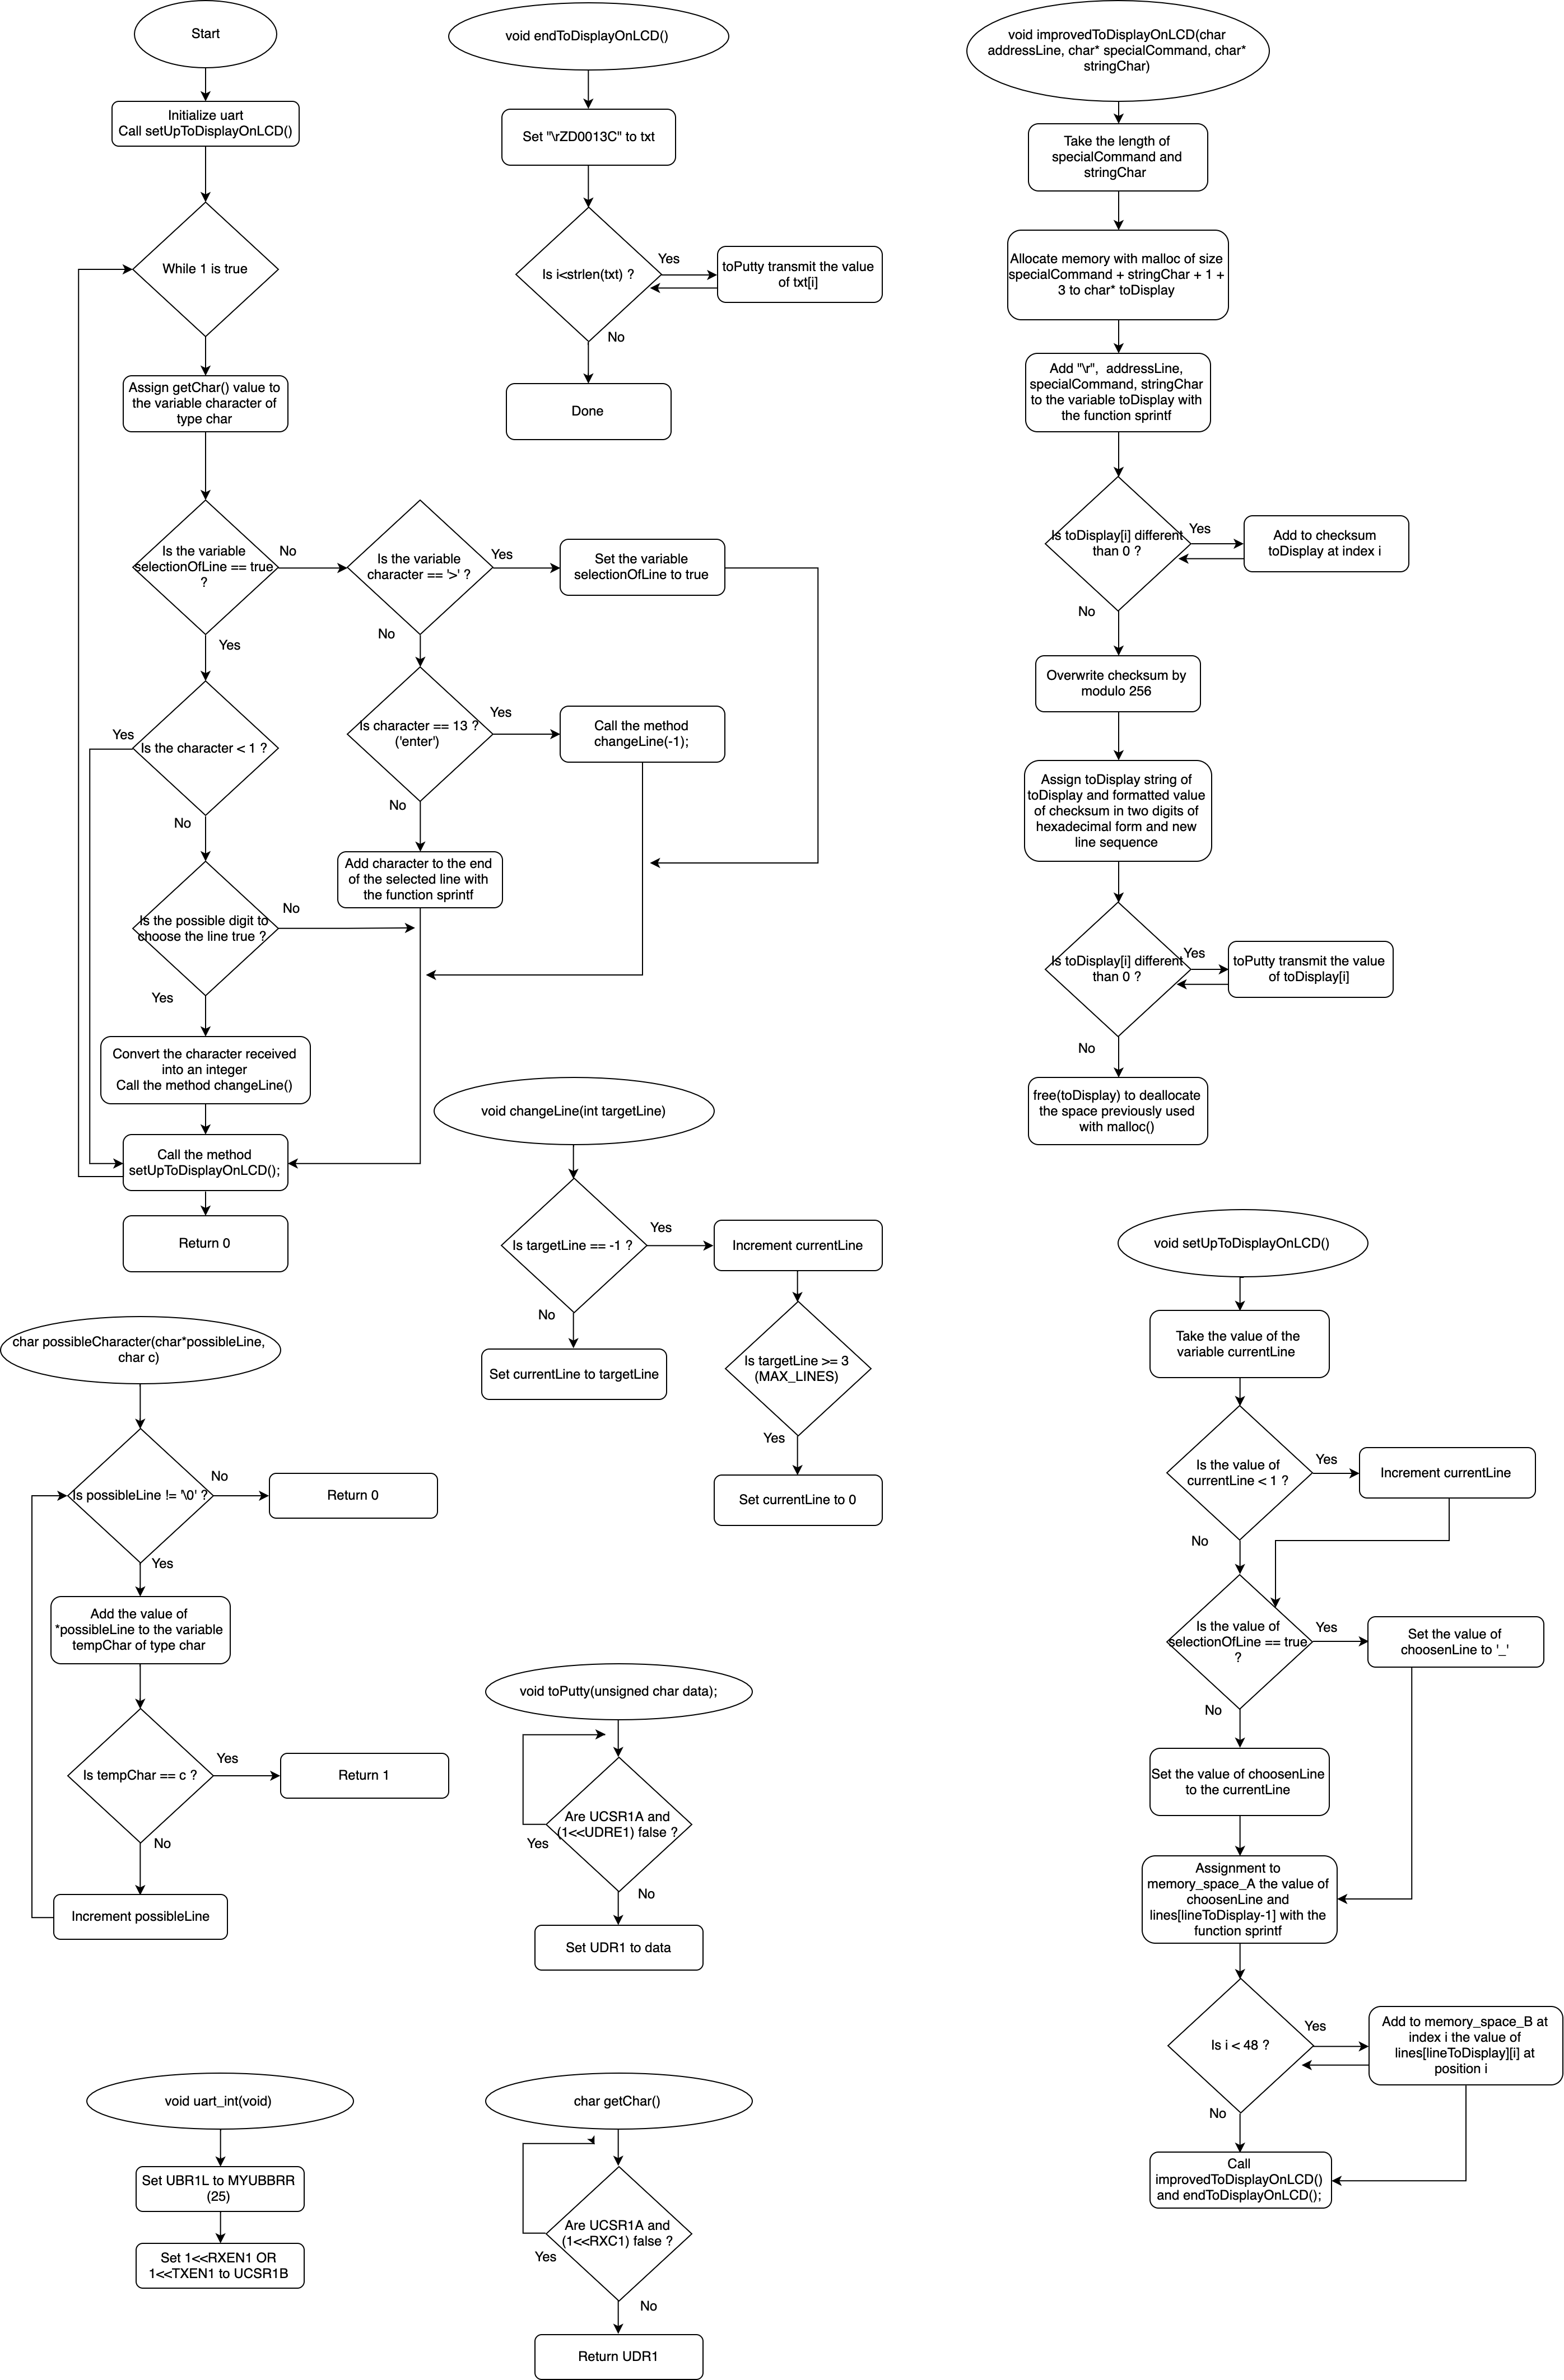
\includegraphics[width=\textwidth/1 ]{flowchart/task4_flowchart.png}
\end{center}
\caption{Task 4 flowchart}
\label{task4}
\end{figure}

\break
%TASK5
\section{Task 5}

\lstset{style=CStyle}

\begin{lstlisting}[style=CStyle]


\end{lstlisting}

\break
\begin{figure}
\begin{center}
%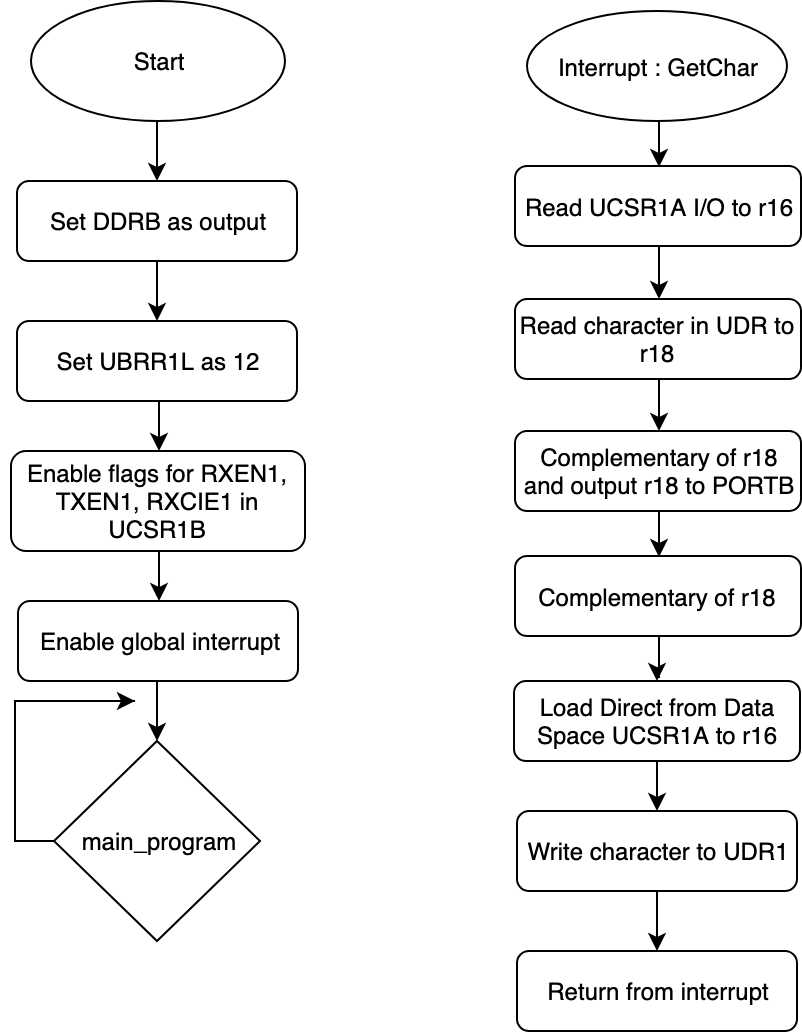
\includegraphics[width=\textwidth/1 ]{flowchart/task5_flowchart.png}
\end{center}
\caption{Task 5 flowchart}
\label{task5}
\end{figure}




% Prints your bibliography database xxx.bib
\bibliographystyle{IEEEtran}
\bibliography{ref.bib}

\end{document}
